
\subsection{Résultats en test}

Voici la liste des résultats obtenus sur le jeu de données de test qui comporte 340 000 (1000 par classe) données:

\begin{center}
\setlength{\tabcolsep}{5mm}
\begin{tabular}{c c c}
\toprule
\textbf{Modèle} & \textbf{Accuracy} & \textbf{MAP@3}  \\



\midrule

\textit{Resnet18} & 77.57&83.78 \\
\textit{Resnet18} données ciblés  &79.58&85.42 \\
Ensemble avec classif  & 75.92 &82.64       \\
Ensemble avec moyenne     & \textbf{79.93}&\textbf{85.66}        \\



\bottomrule
\addlinespace[3mm]
\end{tabular}
\end{center}

On peut voir que l'échantillonnage ciblé du second modèle nous apporte un gain en accuracy d'environ 2\% (de 77.57\% à 79.58\%). C'est un résultat assez intéressant. On peut supposer que cela a permis de gagner un peu en accuracy sur les classes moins bien prédites sans trop affecter celles qui déjà bien classées.


Malheureusement, la modèle par ensemble avec la couche de classification supplémentaire ne donne pas les résultats escomptés, avec une accuracy en test de 75.92\%, c'est le plus faible de tous les modèles essayés.


Le meilleur d'entre tous est le modèle qui fait une moyenne simple des deux premiers modèles avec une accuracy de 79.93\%.


\subsection{Analyse d'erreur}
Il est intéressant de regarder quelques prédictions de notre modèle, cela permet de voir pourquoi il ne fonctionne pas toujours parfaitement. On peut également observer l'accuracy par classe en test pour voir quelles classes fonctionnent moins bien.


Voici un tableau de quelques classes avec une accuracy assez faible (modèle avec échantillons ciblés):
\begin{center}
\begin{tabular}{|c|c|}
\hline
\textbf{Classe} & \textbf{Accuracy} \\ \hline
tornado & 0.142 \\ \hline
birthday cake & 0.254 \\ \hline
guitar & 0.492 \\ \hline
pool & 0.558 \\ \hline
trombone & 0.640 \\ \hline
frog & 0.693 \\ \hline
\end{tabular}
\end{center}



On constate que la plupart de ces classes de dessin de sont évidentes à dessiner et plusieurs techniques peuvent être utilisées pour faire certains de ses dessins. Un humain peut généralement reconnaître le dessin d'un même objet, même si celui est représenté de plusieurs manières différentes (ex: grenouille à la figure \ref{frogs}), ce n'est toutefois pas aussi évident pour réseau de convolution. 

On peut observer des classes ayant bien performées: 

\begin{center}
\begin{tabular}{|c|c|}
\hline
\textbf{Classe} & \textbf{Accuracy} \\ \hline
snowman & 0.953 \\ \hline
star & 0.951 \\ \hline
ladder & 0.951 \\ \hline
envelope & 0.946 \\ \hline
rainbow & 0.931 \\ \hline
clock & 0.924 \\ \hline
\end{tabular}
\end{center}


On constate qu'il s'agit principalement de classes qui sont simples et rapides à dessiner au complet et il n'existe pas plusieurs façons possibles pour dessiner ces dessins, par exemple snowman, star et ladder sont souvent dessinés de la même façon.


On peut également observer quelques mauvaises prédictions de notre modèle sur la figure \ref{comborate}

\begin{figure}[h]
	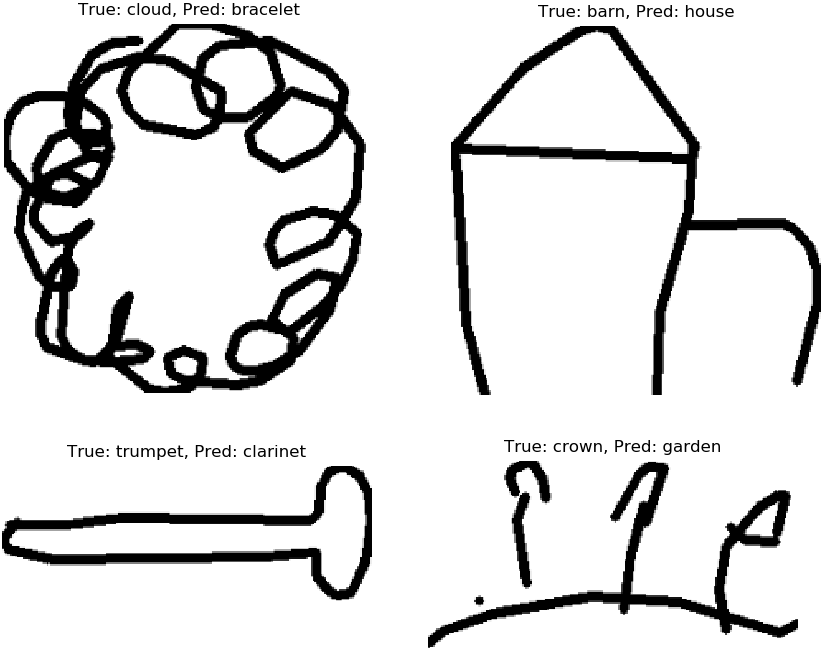
\includegraphics[width=\linewidth]{images/combo_rate.png} % Figure image
	\caption{Images mal prédites} % Figure caption
	\label{comborate} 
\end{figure}

On peut voir que même quand le modèle se trompe, ses prédictions sont quand mêmes représentatives de ce qu'un humain pourrait voir. Par exemple, même si la première image est supposée être un nuage, on peut facilement interpréter ce dessin comme étant un bracelet. 


Même si son accuracy n'est pas si élevé, le modèle nous donne quand même l'impression de performer assez bien étant donné que la plupart de ses prédictions font souvent du sens pour un humain même si elles ne sont pas parfaites. C'est un élément important à garder en tête lorsqu'on veut construire une application réelle en intelligence artificielle.  